\subsection{Power Macromodel for Combinational Logic}



To demonstrate our idea, we will start from a simple design, RISCV-mini~\cite{riscv-mini}.
RISCV-mini implements RV32I of the User-level ISA Version 2.0~\cite{riscv-user-2.0} and
the Machine-level ISA of the Privileged Architecture Version 1.7~\cite{riscv-prev-1.7}.
RISCV-mini includes a 3-stage pipeline as well as instruction and data caches as shown
in Figure~\ref{fig:riscv_mini}, which is neither too simple nor too complex. This is designed
to validate novel ideas before applying them to more complex designs including
RocketChip~\cite{RocketChip}, Hwacha~\cite{Hwacha}, and BOOM~\cite{BOOM}.
We expect that the methodology proposed in this report will accurately predict
the power dissipation of microbenchmarks(median, multiply, qsort, towers, and vvadd) running on RISCV-mini.

\begin{figure*}
	\centering
	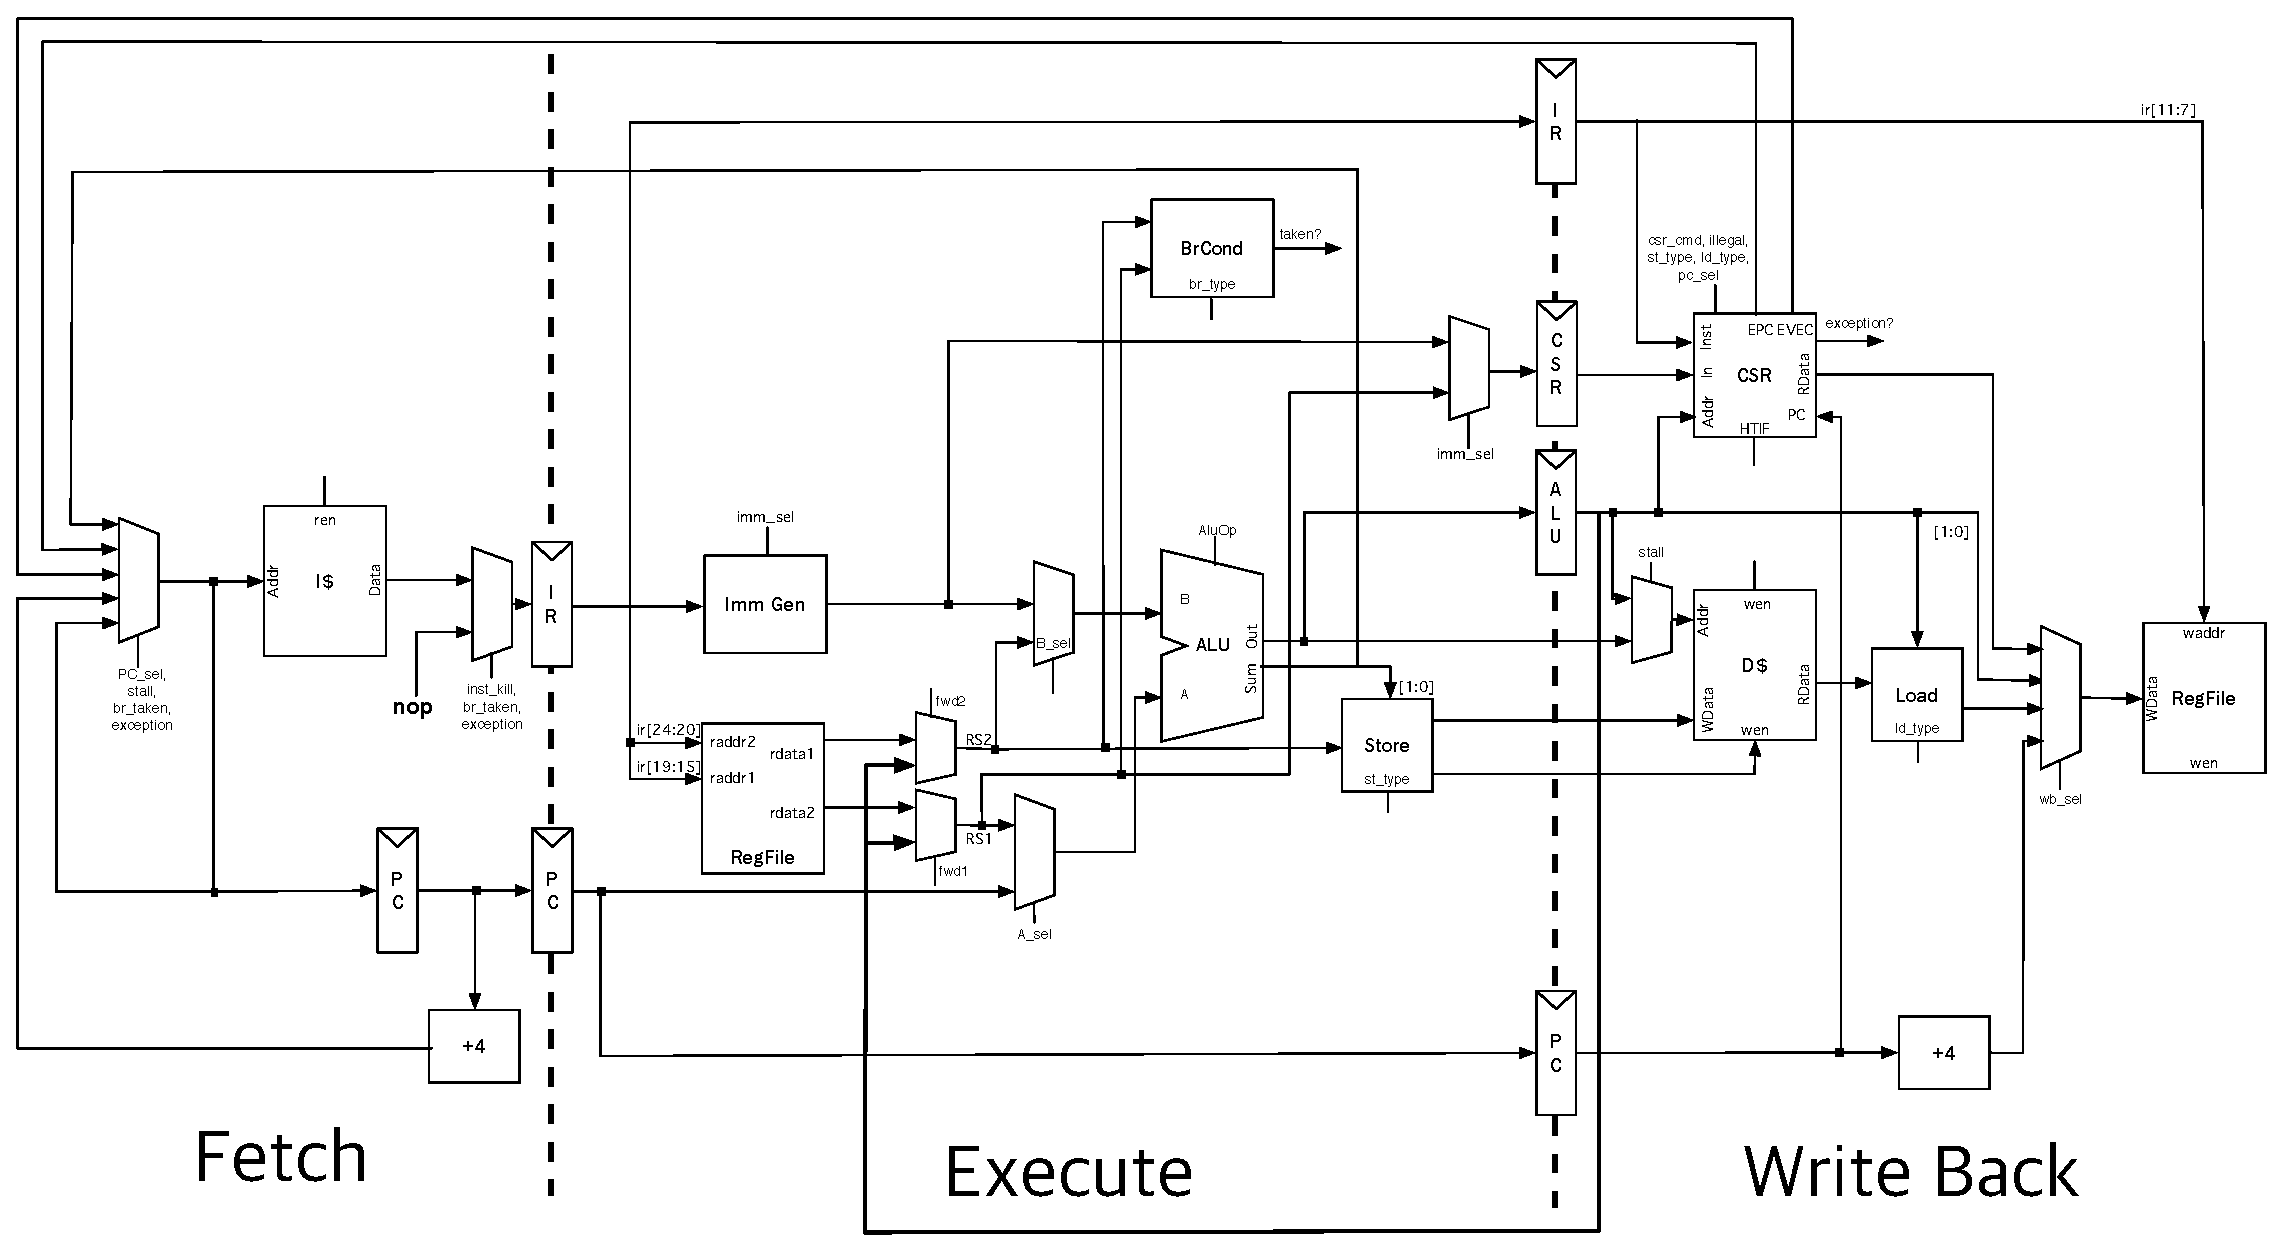
\includegraphics[width=0.85\textwidth,height=\textheight,keepaspectratio]{images/riscv_mini.pdf}
	\caption{RISCV-mini Pipeline}
	\label{fig:riscv_mini}
\end{figure*}